%%%%%%%%%%%%%% Figure 1: 8-K Merging Process
\begin{figure}
	\caption{8-K Merging Process} \label{fig1}
	\begin{center}
		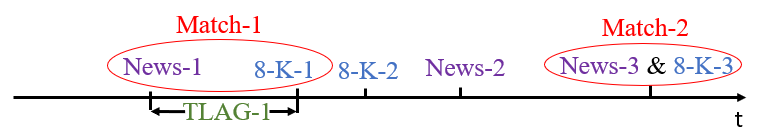
\includegraphics[scale=0.6]{../output/fig/fig1_matching.png}
	\end{center}
\end{figure}

Figure 1 illustrates the 8-K sample matching process. We match every news day to its first subsequent 8-K day, ignoring the successive 8-K days (if any) between two news days (Match-1), or in some cases the 8-K day coincides with news day (Match-2). TLAG is defined as the number of days elapsed between the news release date and 8-K filing date.

%%%%%%%%%%%%%% Figure 2: 8-K Item Distribution
\begin{figure}[htbp]
	\begin{center}
		\caption{8-K Item Distribution} \label{fig2}
		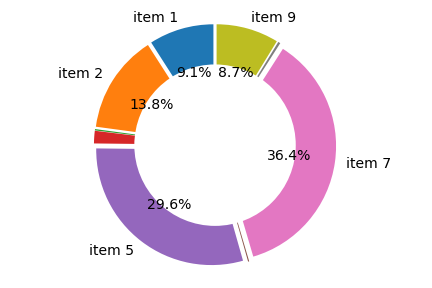
\includegraphics[scale=0.5]{../output/fig/fig2_8-K_before.png}
		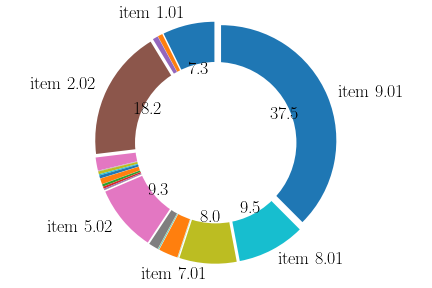
\includegraphics[scale=0.5]{../output/fig/fig2_8-K_after.png}
	\end{center}
\end{figure}

Figure 2 illustrates the 8-K item distribution before (left) and after (right) August 23rd of 2004. Each share of pie chart shows the percentage of corporate events reported under each 8-K items. See 8-K item list in \hyperref[appd]{Appendix D}.